
\section{Inference with unknown exposure status}

\paragraph{}For the known exposure status of an individual, we have shown that \textbf{Algorithm~\ref{alg:metropolis_hastings_inf}} can recover the individual-level infection status, a population-level correlate of protection and the underlying antibody kinetics for two different correlate of protection assumptions and three different levels of individual-level kinetics variability. In practice, this algorithm is unlikely to be useful as the individual-level exposure state is unknown. This section will expand on this algorithm for the case when exposure status is unknown in a serological study. 

\subsection{Overview}

\paragraph{}In the case where the exposure status of each individual, $j$, is unknown, we must now infer their exposure state $E_j \in \{0, 1\}$ and the time of exposure given they are exposed $0 \leq E_j^\tau \leq 120$. In the case where $E_j = 0$, the likelihood is as derived in \textbf{Equation~\ref{ll:1E0}}. However, in the case where $E_j = 1$, the likelihood contains an additional dependency on $E_j^\tau$:

\begin{equation}
L_{E_j = 1}(Y_{j}| Z_j, E_j^\tau, \theta) = \prod_{t \in T_j}P_{obs}(Y_{j,t}|A_{j,t}, \sigma)P_{cop}(Z_j \mid  E^\tau_{j}, \theta)
\end{equation}

where $A_{j,t} = g_{ab}( Z_j,  E_j^\tau, \theta_{ab}, Y^0_i) $.

\subsubsection{Likelihood and priors}

\paragraph{}Let $\mathbf{E} = \{E_0, E_1, \dots, E_{M}\}$ be a vector describing the exposure status of each individual, let $\mathbf{E^{\tau}} = \{E^{\tau}_0, E^{\tau}_1, \dots, E^{\tau}_{n_\mathbf{E}}\}$ be a vector describing the exposure times for each exposed individual. The likelihood of this system is similar to before:

\begin{equation}
\mathcal{L}(\mathbf{Y} | \theta, \mathbf{E}, \mathbf{E^\tau}, \mathbf{Z}) = \prod_{j \in \mathbf{E_0}}L_{E_j = 0}(Y_{j}| \theta) \prod_{j \in \mathbf{E_1}}L_{E_j = 1}(Y_{j}| Z_j, E_j^\tau, \theta) 
\end{equation}

\paragraph{}We now must additionally define priors for $\pi(\mathbf{E})$ and $\pi(\mathbf{E^{\tau}})$. Similar to $\pi(\mathbf{Z})$ we define the prior distribution for  $\pi(\mathbf{E})$ to be a Beta Binomial distribution: $\pi(\mathbf{E}) = \text{BetaBinomial}(n_{\mathbf{E}}| M, 1, 1)$, which is equal to $1/M$ for all $0 \leq n_{\mathbf{E}} \leq M$. For $\pi(\mathbf{E^{\tau}})$, we assume that each element $E_j^\tau \in \mathbf{E^{\tau}}$ has a prior given by $P_t$ such that $\pi(\mathbf{E^{\tau}}) = \prod_{j = 1}^{n_\mathbf{E}} P_t(E_j^\tau)$. The priors for $\pi(\theta)$ and $\pi(\mathbf{Z})$ are as described in \textbf{Section 3}. 
% ILots of questions about this 

\paragraph{}Consequently, we sample from the posterior distribution

\begin{equation}
P(\theta, \mathbf{E}, \mathbf{E^\tau}, \mathbf{Z} | \mathbf{Y}) \propto \mathcal{L}(\mathbf{Y} | \theta, \mathbf{E}, \mathbf{E^\tau}, \mathbf{Z})\pi(\theta)\pi(\mathbf{E})\pi( \mathbf{E^\tau})\pi(\mathbf{Z})
\end{equation}


\paragraph{}If we use a \textbf{Algorithm~\ref{alg:metropolis_hastings_inf}} or any Metropolis Hasting algorithm to infer the exposure status and exposure time, we run into a problem. The number of parameters in the posterior distribution changes according to whether an individual is exposed. Those exposed have parameters $Z_j$ and $E^\tau_j$ to infer, whereas an individual without exposure has neither. Therefore, regardless of the proposal distribution we choose for inferring $\mathbf{E}$, we cannot use the existing algorithm highlighted in \textbf{Algorithm~\ref{alg:metropolis_hastings_inf}} as the detailed balance condition now fails. 


\subsection{The Reversible-Jump MCMC}
The reversible jump Markov chain Monte Carlo (RJ-MCMC) algorithm\cite{Green1995-kh} is a Bayesian statistical method designed for model selection in situations where the number of model parameters can vary. It achieves this by introducing a stochastic mechanism that proposes moves between different models, including adding or removing parameters. The idea is to use a Metropolis-Hastings step to evaluate the acceptance probability of these proposed model changes, ensuring that the Markov chain explores the posterior distribution over both model parameters and model structures. We give a derivation of RJ-MCMC and motivate its use in \textbf{Appendix~\ref{sec:mh2}}.


\subsection{Application of RJ-MCMC to serological data}
\paragraph{}\textbf{Appendix Algorithm~\ref{alg:rjmcmc_A}} is a general framework for jumping from a model $k$ with a parameter values $\theta_k \in \Theta_k$ and another model $k'$ with a parameter values $\theta_{k'} \in \Theta_{k'}$. For our serological inference, our model $k$, represents different elements of the exposure state vector $\mathbf{E} = \{E_0, E_1, \dots, E_{n_\mathbf{E}}\}$ be the number of exposed individuals and $n_\mathbf{E_0} = M - n_\mathbf{E}$ be the number of non-exposed individuals in model $k$. For a given exposure vector $\mathbf{E}_k$, we define three different possible ways to sample a new exposure state vector, $\mathbf{E'}$ in our RJ-MCMC algorithm: a birth event (adding a new exposure), death event (remove an existing exposure), and a move event (exposure state resampled)\cite{Liang2010-oz, Gibson1998-re}. 

\subsubsection{Birth event}

\paragraph{}For a given exposure vector $\mathbf{E}$, a birth event generates a new exposure vector $\mathbf{E'}$, by randomly selecting a non-exposed individual and changing their exposure status from $E_j = 0 \rightarrow E'_j = 1$ and appending it to $\mathbf{E}$. We can derive an expression for $q_k(k' | k)$ by separating into the probability that a birth event is selected at model $k$, $q_{birth}(k' |k)$ and the probability of choosing individual $j$ uniformly from the non-exposed individuals:

\begin{equation}
q_k(k' | k) = q_{birth}(k' |k)\cdot \frac{1}{n_{\mathbf{E_0}}}
\end{equation}

\paragraph{}To understand how to evaluate $q_2(\mathbf{u}'), q_1(\mathbf{u})$ (see \textbf{Appendix~\ref{sec:mh2}}), consider the change in likelihood and the addition prior term for an individual $j$ who is chosen to be exposed:
\begin{equation}
\prod_{t \in T}P_{obs}(Y_{j,t}|Y^0_{j}, \sigma)  \rightarrow  \prod_{t \in T}P_{obs}(Y_{j,t}|A_{j,t}, \sigma)P_{cop}(Z_j \mid Y^0_{j}, \theta)P_t(E_j^t)
\end{equation}

with the likelihood function staying the same for all other individuals. By changing the exposure state for individual $j$, the likelihood now depends on two parameters not in the previous likelihood: the timing of the exposure $E^\tau_j$ and their infection status $Z_j$. In the notation of \textbf{Appendix~\ref{sec:mh2}}, it is convenient to define $\mathbf{u} = (E^\tau_j, Z_j)$. Therefore, we must define a sampling procedure for $\mathbf{u}$ and a probability density function $q_1(\mathbf{u})$ (Note as $d_{k'} > d_k$, we can assume $\mathbf{u'}$ is empty).  For $E^\tau_j$, we sample from the probability density function for the timing $P_t(\cdot)$, and for the infection status, we sample from $P_{cop}(\cdot | Y_j^0, \theta_{cop})$ (see \textbf{Equation~\ref{eq:ll_cop}}). This sampling procedure results in a proposed sample which is in the proposed parameter space $\Theta_{k'}: (\theta_k, E^\tau_j, Z_j) = \theta_{k'} \in \Theta_{k'}$. Consequently, we can choose the identify function for the required bijection $T$ in \textbf{Equation~\ref{eq:T}}, which means the Jacobian is equal to 1.
% maybe show an example where the object is not neat; neg binomial vs poison.
\paragraph{}With this sampling proposal, we can then evaluate $q_1(\mathbf{u})$ through likelihood functions for each of $Z_j$ and $E^\tau_j$:

\begin{equation}
q_1(\mathbf{u}) = q_1(E^\tau_j, Z_j) = P_{cop}(Z_j | E_j^\tau, \theta_{cop})P_t(E^\tau_j)
\end{equation}

\paragraph{}Now let us consider the inverse, which is from the proposed model $k'$ moving back to the model $k$. For this event, we randomly select one person from the proposed exposure state $\mathbf{E'}$ and change their exposure state from $E_j = 1 \rightarrow E'_j = 0$. Similar to above, we derived an expression for $q_k(k | k')$ by separating into the probability that an inverse birth event is selected at model $k$, $q_{birth}(k |k')$ and the probability of choosing individual $j$ uniformly from the exposed individuals of $\mathbf{E}'$:

\begin{equation}
q_k(k | k') = q_{birth}(k |k')\cdot \frac{1}{1 + n_{\mathbf{E}}}
\end{equation}


\paragraph{}In this event, we are removing the parameters $E_j^\tau$ and $Z_j$ from $\theta_{k'}$. After this, we are left with $\theta_k \in \Theta_k$, so we do not need to sample new variables to generate samples from $\Theta_k$. Thus $\mathbf{u}'$ is empty and  $q_2(\mathbf{u}') = 1$. The acceptance ratio for a birth move, where $k = \{\theta, \mathbf{E}, \mathbf{E^\tau}, \mathbf{Z}\} \rightarrow k' = \{\theta, \mathbf{E}', \mathbf{E^\tau}', \mathbf{Z}'\}$ is updated according to a uniformly sampled non-exposed individual $j$:

\begin{equation}
\label{acc:birth}
\alpha(k, k') = \min\left(\frac{P(\theta, \mathbf{E}^{\prime}, \mathbf{E^{\tau \prime}}, \mathbf{Z}^{\prime}, | \mathbf{Y})q_{birth}(k|k^{\prime})n_{\mathbf{E_0}}}{P(\theta, \mathbf{E}, \mathbf{E^{\tau \prime}}, \mathbf{Z}, | \mathbf{Y})P_{cop}(Z_{j}^{\prime} | Y_{j}^{0}, \theta_{cop})P_t(E^{\tau \prime}_j )q_{birth}(k^{\prime} |k)(n_{\mathbf{E}} + 1)} \right)
\end{equation}


\subsubsection{Death event}


\paragraph{}For a given exposure vector $\mathbf{E}$, a death event generates a new exposure vector $\mathbf{E'}$, by randomly selecting an exposed individual and changing their exposure status from $E_j = 1 \rightarrow E'_j = 0$ therefore removing it from $\mathbf{E}$. We can derive an expression for $q_k(k' | k)$ by separating into the probability that a death event is selected at model $k$, $q_{death}(k' |k)$ and the probability of choosing individual $j$ uniformly from the exposed individuals:

\begin{equation}
q_k(k' | k) = q_{death}(k' |k)\cdot \frac{1}{n_{\mathbf{E}}}
\end{equation}

The reverse probability $q_k(k^{\prime} | k)$ is equivalent to a birth event, that is, the probability of sampling a non-exposed person in $\mathbf{E}'$, or 

\begin{equation}
q_k(k | k') = q_{death}(k | k')\cdot \frac{1}{1 + n_{\mathbf{E_0}}}
\end{equation}


\paragraph{}To understand how to evaluate $q_1(\mathbf{u)}, q_2(\mathbf{u}')$, consider the change in likelihood for an individual $j$ who is chosen to be exposed:
\begin{equation}
 \prod_{t \in T}P_{obs}(Y_{j,t}|A_{j,t}, \sigma)P_{cop}(Z_j \mid  Y^0_{j}, \theta)P_t(E_j^\tau) \rightarrow \prod_{t \in T}P_{obs}(Y_{j,t}|Y^0_{j}, \sigma) 
\end{equation}

with the likelihood function staying the same for all other individuals. By changing the exposure state for individual $j$, the likelihood now depends on two fewer parameters than were in the previous likelihood for $k'$: the timing of the exposure $E^\tau_j$ and their infection status $Z_j$. Therefore, by using the same argument as in the 'birth event' section, defining $q_1(\mathbf{u}) = 1$ and $q_2(\mathbf{u}') = P_t(E^\tau_j)P_{cop}(Z_j | E_j^\tau, \theta_{cop})$, we can take the identity bijection as sample a value in state $\theta' \in \Theta'$ directly.  The acceptance ratio for a death event, where our current state is $k = \{\theta, \mathbf{E}, \mathbf{E^\tau}, \mathbf{Z}\} \rightarrow k' = \{\theta, \mathbf{E}', \mathbf{E^\tau}', \mathbf{Z}'\}$ is updated according to a uniformly sampled exposed individual $j$:

\begin{equation}
\label{acc:death}
\alpha(k, k^{\prime}) = \min\left(\frac{P(\theta, \mathbf{E}^{\prime}, \mathbf{E^{\tau}}^{\prime}, \mathbf{Z}, | \mathbf{Y})P_{cop}(Z_{j} | E_{j}, \theta_{cop})P_t(E^\tau_j)q_{death}(k|k^{\prime})n_{\mathbf{E}}}{P(\theta, \mathbf{E}, \mathbf{E^{\tau}}, \mathbf{Z}, | \mathbf{Y})q_{death}(k^{\prime}|k)(n_{\mathbf{E_0}} + 1)} \right)
\end{equation}

\subsubsection{Move event}

If we use only the birth and death event highlighted above, the timing of the exposures, $\mathbf{E^\tau}$ is not efficiently explored.\cite{Gibson1998-re} Therefore, it is desirable that values of $\mathbf{E^\tau}$ can be explored for fixed values of $\mathbf{Z}$, and $\mathbf{E}$. Therefore, we define a move event which resamples a proportion of the $\mathbf{E}^{\tau}$, and for each individual, we sample a new time $E_{j'}^\tau$ from the proposal distribution

$$E_{j'}^{\tau} \sim q_t(E_{j}^{\tau}) $$

where we choose the proposal to be the symmetric $q_t(E_{j}^{\tau}) = \mathcal{N}(E_j^{t, (i)}, \sigma^{(i)}_j)$.  Where $\sigma^{(i)}_j$ is an adaptively updated standard deviation for the proposal for the normal, which updates according to the regime:

$$\log\left(\sigma^{(i + 1)}_j\right) = \log\left(\sigma^{(i)}_j\right) +  (1 + i)^{-0.5}*(\alpha - 0.44) $$

where $\alpha$ is the metropolis hasting ratio for $E_{j'}^{\tau}$ vs $E_j^{\tau, (i)}$.

With these three moves, we define the RJ-MCMC algorithm (\textbf{Algorithm~\ref{alg:rjmcmc_B}}), which effectively samples values from $\{\theta$, $\mathbf{E}$, $\mathbf{E_\tau}$, $\mathbf{Z}\}$. 


\paragraph{Note on $q_{birth}$, $q_{death}$, $q_{par}$:} We can select values $q_{birth}(k' | k)$ and $q_{death}(k' | k)$ which simplify the expression in the acceptance ratios in \textbf{Equation~\ref{acc:birth}} and \textbf{Equation~\ref{acc:death}}. If $k$ is such that $n_{\mathbf{E}} = 0$, then we choose $q_{par} = 1/3$ and $q_{birth} = 2/3$. If  $n_{\mathbf{E}} = M$, then we choose $q_{par} = 1/3$ and $q_{death} = 2/3$. Otherwise, we  $q_{birth}(k' | k) = q_{death}(k' | k) = q_{par} = 1/3$ for all $k'$. Choosing these values means that the values of $q_{birth}$, $q_{death}$, and $q_{par}$ cancel in all acceptance ratios (\textbf{Equation~\ref{acc:birth}} and \textbf{Equation~\ref{acc:death}}) for all values of $k'$ given $k$.

\paragraph{} An algorithm describing the Birth-Death RJ-MCMC algorithm for this data is given in \textbf{Algorithm~\ref{alg:rjmcmc_B}}.

\begin{algorithm}[H]
\caption{Birth-Death Reversible Jump MCMC Algorithm}
\label{alg:rjmcmc_B}
\begin{algorithmic}[1]
    \State Chose a model $k$ and initialize the chain with an initial states $\theta^{(0)}_{k}$, $\mathbf{E^{(0)}}$, $\mathbf{E^{\tau, (0)}}$ and $\mathbf{Z^{(0)}}$. If $0 < n_\mathbf{E} < M$, then $p_{birth} = p_{death} = p_{par} = 0.33$; if $n_\mathbf{E} = 0$, $p_{birth} = 0.67, p_{par} = 0.33, p_{death} = 0$; if $n_\mathbf{E} = M$, $p_{death} = 0.67, p_{par} = 0.33, p_{birth} = 0$.
    \For{$i = 1$ to $N$}
   	\State Sample a candidate state $\theta' \sim q_\theta(\theta^{(i)}, \psi^{(i)}_{adapt})$
    	\State $u_1 \sim \mathcal{U}(0, 1)$  
	 \If{$u_1 \leq p_{birth}$}
	 	\State \textit{Birth move}. Select $j' \in \mathbf{E^{(i)}_0}$, set $E_{j'} = 1$, sample $E^\tau_{j'} \sim P_t(\cdot)$, $Z_{j'}\sim P_{cop}(\cdot | Y_{j'}^0, \theta_{cop})$ and update $\{\theta^{(i)}, \mathbf{E^{(i)}}, \mathbf{E^{\tau, (i)}}, \mathbf{Z^{(i)}}\} \rightarrow \{\theta', \mathbf{E}', \mathbf{E^\tau}', \mathbf{Z}'\}$. Then, calculate the acceptance probability 
		$$\alpha(k^{(i)}, k') = \min\left(\frac{P(\theta', \mathbf{E}', \mathbf{E^\tau}', \mathbf{Z}', | \mathbf{Y})n_{\mathbf{E_0}}}{P(\theta, \mathbf{E^{(i)}}, \mathbf{E^{\tau, (i)}}, \mathbf{Z^{(i)}}, | \mathbf{Y})P_{cop}(Z_{j'} | E_{j'}, \theta_{cop})P_t(E^\tau_{j'})(n_{\mathbf{E}} + 1)} \right)$$
	\ElsIf{$u_1 \leq (p_{birth} + p_{death})$}	
		\State \textit{Death move}. Select $j' \in \mathbf{E^{(i)}_1}$, set $E_{j'} = 0$ and update $\{\theta^{(i)}, \mathbf{E^{(i)}}, \mathbf{E^{\tau, (i)}}, \mathbf{Z^{(i)}}\} \rightarrow \{\theta', \mathbf{E}', \mathbf{E^\tau}', \mathbf{Z}'\}$. Then calculate the acceptance probability 
$$\alpha(k^{(i)}, k') = \min\left(\frac{P(\theta', \mathbf{E}', \mathbf{E^{\tau}}', \mathbf{} Z| \mathbf{Y})P_{cop}(Z_{j'} | E_{j'}, \theta_{cop})P_t(E^\tau_{j'})n_{\mathbf{E}}}{P(\theta, \mathbf{E^{(i)}}, \mathbf{E^{\tau, (i)}}, \mathbf{Z^{(i)}}, | \mathbf{Y})(n_{\mathbf{E_0}} + 1)} \right)$$
	\Else
        \State Select $j' \in N_{E = 1}$ and resample from the proposal $E_{j'}^{\tau} \sim \mathcal{N}\left(E_{j}^{\tau, (i)}, \sigma^{(i)}_{j}\right)$ and update $\mathbf{E^{t, (i)}} \rightarrow \mathbf{E^{t, *}}$
    	    \State Compute the acceptance ratio:
        		\[
        \alpha(k^{(i)}, k') = \min\left(1, \frac{P(\theta', \mathbf{E}', \mathbf{E^{\tau}}', \mathbf{Z}'|\mathbf{Y})}{P(\theta^{(i)}, \mathbf{E^{(i)}}, \mathbf{E^{\tau, (i)}}, \mathbf{Z}^{(i)}|\mathbf{Y})} \right)
        			\]
	\State Update $ \psi^{(i + 1)}_{adapt} \leftarrow \psi^{(i)}_{adapt}$ and $\sigma_j^{i + 1} \leftarrow \sigma_j^{i}$
        \EndIf 
		   \State Sample $u \sim \mathcal{U}(0, 1)$
		       \If{$u \leq \alpha$}
            			\State Accept the candidate state: Let $\{\theta^{(i+1)}, \mathbf{E^{(i+1)}}, \mathbf{E^{\tau, (i+1)}}, \mathbf{Z^{(i+1)}}\} \leftarrow \{\theta', \mathbf{E}', \mathbf{E^\tau}', \mathbf{Z}'\}$
			\Else
				\State Reject the candidate state: Let $\{\theta^{(i+1)}, \mathbf{E^{(i+1)}}, \mathbf{E^{\tau, (i+1)}}, \mathbf{Z^{(i+1)}}\} \leftarrow \{\theta^{(i)}, \mathbf{E^{(i)}}, \mathbf{E^{\tau, (i)}}, \mathbf{Z^{(i)}}\}$

			\EndIf        

    \EndFor
\end{algorithmic}
\end{algorithm}

\paragraph{Note on prior distributions}As M is fixed, then $\pi(\mathbf{E}) = 1/M$ for all $0 \leq n_{\mathbf{E}} \leq M$ and thus cancels out in the acceptance ratio for the birth, death and parameter update move. $\pi(\mathbf{Z})$ cancels out in the parameter updating acceptance ratio (as described in \textbf{Algorithm~\ref{alg:metropolis_hastings_inf}}. However, in the birth and death move, as $n_{\mathbf{E}}$ in the current state and $n_{\mathbf{E}'}$ is the proposed state have different values, then $\pi(\mathbf{Z}) = 1/n_\mathbf{E_1} \neq  1/n_\mathbf{E_1'} = \pi(\mathbf{Z}')$ no longer cancels in the ratio and must be included to ensure the detailed balance condition holds. 
We choose a non-informative for the timing of infection given exposure prior: $P_t(E_j^\tau) = 1 / 120$.

\subsection{Implementation }
\paragraph{}  \textbf{Algorithm~\ref{alg:rjmcmc_B}} is coded manually in R and C++ through Rcpp. We run the algorithm for four chains, each with 400,000 steps and 200,000 burn-in steps. The initial values for $\theta$, $\mathbf{Z}$, $\mathbf{E}$, and $\mathbf{E^{\tau}}$ are sampled from their prior distributions. We initialise the adaptive covariance by running with an identity matrix with each parameter scale according to 1,000 steps, then sample from the adaptive scheme. We thin the posterior samples by taking one in every 100, leaving 2,000 posterior samples at the end of the sampling. The trace plots for each of the six model fits are given in \textbf{Appendix Figure~\ref{app_traceB}}.

\paragraph{}Through \textbf{Algorithm~\ref{alg:rjmcmc_B}} we define an efficient sampling procedure for the state space $k = \{\theta, \mathbf{E}, \mathbf{E^\tau}, \mathbf{Z}\}$ within one single framework. This allows us to infer the exposure state, infection state, exposure and infection timings across the epidemic, the correlates of protection and the antibody kinetics function. We show the ability of this procedure to recover our simulated data displayed in the next section.

\subsection{Simulation recovery }
\paragraph{}After running \textbf{Algorithm~\ref{alg:rjmcmc_B}}, we plot the posterior samples, $\hat{\theta}$, $\hat{\mathbf{Z}}$,  $\hat{\mathbf{E}}$, and  $\hat{\mathbf{E}^\tau}$ and compare with the simulated parameters.

\subsubsection{Exposure state recovery}
\paragraph{} \textbf{Algorithm~\ref{alg:rjmcmc_B}} can recover the population-level exposure rates across all six models (\textbf{Figure~\ref{fit2:exp}}). For Model A (no COP), we consistently overestimated the number of individuals exposed (estimating between 135 (95\% CrI 120–151) exposures when 122 were simulated). However, the exposure state effectively acts as a nuisance parameter in the recovery of the COP as the probability someone is exposed is irrelevant once you condition on exposure, and we see that the COP function is still consistently recovered (see \textbf{Figure~\ref{fit2:cop}}) % Something about nuisance parameters

\begin{figure}[H]

    \centering
    \begin{subfigure}{0.31\textwidth}
        \centering
        \includegraphics[width=\textwidth]{\myimagepath/outputs/fits/cesNoCOP_notd/inferExp/figs/obs_0.1/exposure_recov.png}
        \caption{No COP, 10\% variability \label{fit1:inf}}
    \end{subfigure}
    \begin{subfigure}{0.31\textwidth}
        \centering
        \includegraphics[width=\textwidth]{\myimagepath/outputs/fits/cesNoCOP_notd/inferExp/figs/obs_0.3/exposure_recov.png}
        \caption{No COP, 30\% variability}
    \end{subfigure}
    \begin{subfigure}{0.31\textwidth}
        \centering
        \includegraphics[width=\textwidth]{\myimagepath/outputs/fits/cesNoCOP_notd/inferExp/figs/obs_0.5/exposure_recov.png}
        \caption{No COP, 50\% variability}
    \end{subfigure}
    
  \begin{subfigure}{0.31\textwidth}
        \centering
        \includegraphics[width=\textwidth]{\myimagepath/outputs/fits/cesCOP_notd/inferExp/figs/obs_0.1/exposure_recov.png}
        \caption{ COP, 10\% variability}
    \end{subfigure}
    \begin{subfigure}{0.31\textwidth}
        \centering
        \includegraphics[width=\textwidth]{\myimagepath/outputs/fits/cesCOP_notd/inferExp/figs/obs_0.3/exposure_recov.png}
        \caption{ COP, 30\% variability}
    \end{subfigure}
    \begin{subfigure}{0.31\textwidth}
        \centering
        \includegraphics[width=\textwidth]{\myimagepath/outputs/fits/cesCOP_notd/inferExp/figs/obs_0.5/exposure_recov.png}
        \caption{ COP, 50\% variability}
    \end{subfigure}
    
    \caption{Simulation recovery of exposure status $\hat{E}$ and epidemic curve for two COP models (top: No COP, bottom: logistic COP) and three different levels antibody kinetics variability (10\%, 30\%, 50\%) \label{fit2:exp}. Red lines in B figures show the true number of exposures from the simulations }
\end{figure}


\subsubsection{Exposure times recovery}
\paragraph{} \textbf{Algorithm~\ref{alg:rjmcmc_B}} can recover the exposure times. The posterior of the exposure times for individual $j$ is given by $\hat{E^\tau_j}$ and plotted with the simulated exposure time in \textbf{Figure~\ref{fit2:exp_time} } by their exposure status. For those infected, the model can reasonably recover the exposure times for each individual, though as the antibody kinetics variability increases, the exposure time becomes less recoverable. For example, for Model A (no COP), the proportion of individuals with infection times inferred within 14 days of their simulated infection day is 97\%, 84\%, and 73\% for 10\%, 30\% and 50\% variability, respectively(\textbf{Figure~\ref{fit2:exp_time_error}}). For all six models, the epidemic curve is reasonably recovered (\textbf{Figure~\ref{fit2:exp_time}}). 
\begin{figure}[H]

    \centering
    \begin{subfigure}{0.31\textwidth}
        \centering
        \includegraphics[width=\textwidth]{\myimagepath/outputs/fits/cesNoCOP_notd/inferExp/figs/obs_0.1/exposure_time_recov.png}
        \caption{No COP, 10\% variability \label{fit1:inf}}
    \end{subfigure}
    \begin{subfigure}{0.31\textwidth}
        \centering
        \includegraphics[width=\textwidth]{\myimagepath/outputs/fits/cesNoCOP_notd/inferExp/figs/obs_0.3/exposure_time_recov.png}
        \caption{No COP, 30\% variability}
    \end{subfigure}
    \begin{subfigure}{0.31\textwidth}
        \centering
        \includegraphics[width=\textwidth]{\myimagepath/outputs/fits/cesNoCOP_notd/inferExp/figs/obs_0.5/exposure_time_recov.png}
        \caption{No COP, 50\% variability}
    \end{subfigure}
    
  \begin{subfigure}{0.31\textwidth}
        \centering
        \includegraphics[width=\textwidth]{\myimagepath/outputs/fits/cesCOP_notd/inferExp/figs/obs_0.1/exposure_time_recov.png}
        \caption{ COP, 10\% variability}
    \end{subfigure}
    \begin{subfigure}{0.31\textwidth}
        \centering
        \includegraphics[width=\textwidth]{\myimagepath/outputs/fits/cesCOP_notd/inferExp/figs/obs_0.3/exposure_time_recov.png}
        \caption{ COP, 30\% variability}
    \end{subfigure}
    \begin{subfigure}{0.31\textwidth}
        \centering
        \includegraphics[width=\textwidth]{\myimagepath/outputs/fits/cesCOP_notd/inferExp/figs/obs_0.5/exposure_time_recov.png}
        \caption{ COP, 50\% variability}
    \end{subfigure}
    
    \caption{Simulation recovery of exposure and infection timings $\hat{E^\tau}$ and epidemic curve for two COP models (top: No COP, bottom: logistic COP) and three different levels antibody kinetics variability (10\%, 30\%, 50\%) \label{fit2:exp_time}}
\end{figure}


\begin{figure}[H]

    \centering
    \begin{subfigure}{0.31\textwidth}
        \centering
        \includegraphics[width=\textwidth]{\myimagepath/outputs/fits/cesNoCOP_notd/inferExp/figs/obs_0.1/exposure_time_recov_error.png}
        \caption{No COP, 10\% variability \label{fit1:inf}}
    \end{subfigure}
    \begin{subfigure}{0.31\textwidth}
        \centering
        \includegraphics[width=\textwidth]{\myimagepath/outputs/fits/cesNoCOP_notd/inferExp/figs/obs_0.3/exposure_time_recov_error.png}
        \caption{No COP, 30\% variability}
    \end{subfigure}
    \begin{subfigure}{0.31\textwidth}
        \centering
        \includegraphics[width=\textwidth]{\myimagepath/outputs/fits/cesNoCOP_notd/inferExp/figs/obs_0.5/exposure_time_recov_error.png}
        \caption{No COP, 50\% variability}
    \end{subfigure}
    
  \begin{subfigure}{0.31\textwidth}
        \centering
        \includegraphics[width=\textwidth]{\myimagepath/outputs/fits/cesCOP_notd/inferExp/figs/obs_0.1/exposure_time_recov_error.png}
        \caption{ COP, 10\%variability}
    \end{subfigure}
    \begin{subfigure}{0.31\textwidth}
        \centering
        \includegraphics[width=\textwidth]{\myimagepath/outputs/fits/cesCOP_notd/inferExp/figs/obs_0.3/exposure_time_recov_error.png}
        \caption{ COP, 30\% variability}
    \end{subfigure}
    \begin{subfigure}{0.31\textwidth}
        \centering
        \includegraphics[width=\textwidth]{\myimagepath/outputs/fits/cesCOP_notd/inferExp/figs/obs_0.5/exposure_time_recov_error.png}
        \caption{ COP, 50\% variability}
    \end{subfigure}
    
    \caption{Error in estimating infection time two COP models (top: No COP, bottom: logistic COP) and three different levels antibody kinetics variability (10\%, 30\%, 50\%) \label{fit2:exp_time_error}}
\end{figure}

% JH: Suggestions:
%1. Remove the y-axis labels and maybe even the plot.grid. The reader doesn't really care about the individual IDs.
%2. Suggest using a different way of showing "posterior probability of exposure", maybe by color scale rather than alpha.
%3. Do you think there's a way to indicate which infection timings are within the 95% CrI and which are wrong? Maybe grouping by true positive, true negative, false positive and false negative?
% What are the plots labeled B in each scenario? Is this the epidemic curve? Suggest more informative y-axis labels


\subsubsection{Infection state recovery}

\paragraph{}We also recover the infection status of each individual from the simulated data. Suppose the set posterior samples of the infection status for individual $j$ is given by $\hat{Z_j} $. In that case, we plot the expectation $\mathbb{E}(\hat{Z_j} )$ so we can assess the ability of the algorithm to recover the individual-level simulated infection status (\textbf{Figure~\ref{fit2:inf}}). Nearly all infection states are accurately recovered for all six models. 

\begin{figure}[H]
    \centering
    \begin{subfigure}{0.31\textwidth}
        \centering
        \includegraphics[width=\textwidth]{\myimagepath/outputs/fits/cesNoCOP_notd/inferExp/figs/obs_0.1/infection_recov.png}
        \caption{No COP, 10\% variability \label{fit1:inf}}
    \end{subfigure}
    \begin{subfigure}{0.31\textwidth}
        \centering
        \includegraphics[width=\textwidth]{\myimagepath/outputs/fits/cesNoCOP_notd/inferExp/figs/obs_0.3/infection_recov.png}
        \caption{No COP, 30\% variability}
    \end{subfigure}
    \begin{subfigure}{0.31\textwidth}
        \centering
        \includegraphics[width=\textwidth]{\myimagepath/outputs/fits/cesNoCOP_notd/inferExp/figs/obs_0.5/infection_recov.png}
        \caption{No COP, 50\% variability}
    \end{subfigure}
    
  \begin{subfigure}{0.31\textwidth}
        \centering
        \includegraphics[width=\textwidth]{\myimagepath/outputs/fits/cesCOP_notd/inferExp/figs/obs_0.1/infection_recov.png}
        \caption{ COP, 10\% variability}
    \end{subfigure}
    \begin{subfigure}{0.31\textwidth}
        \centering
        \includegraphics[width=\textwidth]{\myimagepath/outputs/fits/cesCOP_notd/inferExp/figs/obs_0.3/infection_recov.png}
        \caption{ COP, 30\% variability}
    \end{subfigure}
    \begin{subfigure}{0.31\textwidth}
        \centering
        \includegraphics[width=\textwidth]{\myimagepath/outputs/fits/cesCOP_notd/inferExp/figs/obs_0.5/infection_recov.png}
        \caption{ COP, 50\% variability}
    \end{subfigure}
    
    \caption{Simulation recovery of the individual infection status, $\hat{Z_j}$, for two COP models (top: No COP, bottom: logistic COP) and three different levels antibody kinetics variability (10\%, 30\%, 50\%) \label{fit2:inf}}
\end{figure}

\subsubsection{Correlate of protection}

\paragraph{} \textbf{Algorithm~\ref{alg:rjmcmc_B}} performs well at recovering the correlate of protection function $f_{cop}(x, \hat{\theta}_{cop})$, where $x$ is the titre value at infection and where $\hat{\theta}_{cop} = \{\hat{\beta_0}, \hat{\beta_1}\}$ are the posterior samples for $\beta_0$ and $\beta_1$. For Model A, we find that the COP curve is recovered, with the simulated line within a 50\% confidence interval of the posterior sample (\textbf{Figure~\ref{fit2:cop}}). For Model B, we find the logistic shape of the COP is recovered in the posterior samples. 

\begin{figure}[H]

    \centering
    \begin{subfigure}{0.31\textwidth}
        \centering
        \includegraphics[width=\textwidth]{\myimagepath/outputs/fits/cesNoCOP_notd/inferExp/figs/obs_0.1/cop_recov.png}
        \caption{No COP, 10\% variability}
    \end{subfigure}
    \begin{subfigure}{0.31\textwidth}
        \centering
        \includegraphics[width=\textwidth]{\myimagepath/outputs/fits/cesNoCOP_notd/inferExp/figs/obs_0.3/cop_recov.png}
        \caption{No COP, 30\% variability}
    \end{subfigure}
    \begin{subfigure}{0.31\textwidth}
        \centering
        \includegraphics[width=\textwidth]{\myimagepath/outputs/fits/cesNoCOP_notd/inferExp/figs/obs_0.5/cop_recov.png}
        \caption{No COP, 50\% variability}
    \end{subfigure}
    
  \begin{subfigure}{0.31\textwidth}
        \centering
        \includegraphics[width=\textwidth]{\myimagepath/outputs/fits/cesCOP_notd/inferExp/figs/obs_0.1/cop_recov.png}
        \caption{ COP, 10\% variability}
    \end{subfigure}
    \begin{subfigure}{0.31\textwidth}
        \centering
        \includegraphics[width=\textwidth]{\myimagepath/outputs/fits/cesCOP_notd/inferExp/figs/obs_0.3/cop_recov.png}
        \caption{ COP, 30\% variability}
    \end{subfigure}
    \begin{subfigure}{0.31\textwidth}
        \centering
        \includegraphics[width=\textwidth]{\myimagepath/outputs/fits/cesCOP_notd/inferExp/figs/obs_0.5/cop_recov.png}
        \caption{ COP, 50\% variability}
    \end{subfigure}
    
    \caption{Simulation recovery of the COP function, posterior samples plot  $f_{cop}(x, \hat{\theta}_{cop})$. We have two different COp models (top: No COP, bottom: logistic COP) and three different levels of antibody kinetics variability (10\%, 30\%, 50\%). \label{fit2:cop}}
\end{figure}

% AK: Nice. Might be worth making the point clearly somewhere that if we’re interested in COP, arguably everything else (antibody kinetics, infection rates) are basically nuisance parameters, and it might not matter much if they have marginal uncertainty if when we aggregate across dynamics to get COP the estimates are good?


\subsubsection{Antibody kinetics}
\paragraph{} \textbf{Algorithm~\ref{alg:rjmcmc_B}} also recovers the simualted antibody kinetics. Let us plot $f_{ab}(s, \hat{a}, \hat{b}, \hat{c})$, the posterior predictive distribution for the antibody kinetic boosting, given posterior distributions for $\hat{a}, \hat{b}$, and $\hat{c}$. For all six models, the some of the posterior distributions for $\hat{a}, \hat{b}$, and $\hat{c}$ differ slightly from the simulated value. However, despite this, the recovered mean trajectory seems to well represent the individual-level kinetics from the simulated data (\textbf{Figure~\ref{fit2:ab}}). 

\begin{figure}[H]

    \centering
    \begin{subfigure}{0.31\textwidth}
        \centering
        \includegraphics[width=\textwidth]{\myimagepath/outputs/fits/cesNoCOP_notd/inferExp/figs/obs_0.1/ab_kinetics_recov.png}
        \caption{No COP, 10\% variability}
    \end{subfigure}
    \begin{subfigure}{0.31\textwidth}
        \centering
        \includegraphics[width=\textwidth]{\myimagepath/outputs/fits/cesNoCOP_notd/inferExp/figs/obs_0.3/ab_kinetics_recov.png}
        \caption{No COP, 30\% variability}
    \end{subfigure}
    \begin{subfigure}{0.31\textwidth}
        \centering
        \includegraphics[width=\textwidth]{\myimagepath/outputs/fits/cesNoCOP_notd/inferExp/figs/obs_0.5/ab_kinetics_recov.png}
        \caption{No COP, 50\% variability}
    \end{subfigure}
    
  \begin{subfigure}{0.31\textwidth}
        \centering
        \includegraphics[width=\textwidth]{\myimagepath/outputs/fits/cesCOP_notd/inferExp/figs/obs_0.1/ab_kinetics_recov.png}
        \caption{ COP, 10\% variability}
    \end{subfigure}
    \begin{subfigure}{0.31\textwidth}
        \centering
        \includegraphics[width=\textwidth]{\myimagepath/outputs/fits/cesCOP_notd/inferExp/figs/obs_0.3/ab_kinetics_recov.png}
        \caption{ COP, 30\% variability}
    \end{subfigure}
    \begin{subfigure}{0.31\textwidth}
        \centering
        \includegraphics[width=\textwidth]{\myimagepath/outputs/fits/cesCOP_notd/inferExp/figs/obs_0.5/ab_kinetics_recov.png}
        \caption{ COP, 50\% variability}
    \end{subfigure}
    
    \caption{Simulation recovery of the antibody kinetics function with posterior samples plot $f^1_{ab}(s, \hat{a}, \hat{b}, \hat{c})$. We have two different COP models (top: No COP, bottom: logistic COP) and three different levels of antibody kinetics variability (10\%, 30\%, 50\%). \label{fit2:ab}}
   \end{figure}
  